\documentclass[a4paper, 12pt]{article}

\renewcommand{\familydefault}{\sfdefault}

\usepackage[english]{babel}
\usepackage{amsmath}
\usepackage{amssymb}
\usepackage{parskip}
\usepackage{graphicx}
\graphicspath{ {./images/} }
\usepackage{capt-of}

\begin{document}
\title{\Large{\textbf{Machine Learning Algebra}}}
\author{By Matthieu Lagarde}
\date{April 9, 2022}

\maketitle

\setcounter{page}{2}

\newpage
\section{Multivariate linear regression}
\subsection{Notations}

Let $m$ be the number of examples or observations in our training set. Let $n$ be the number of features or explanatory variables observed for each example of the training set. Let $x_j^{(i)}$ be the value of feature $j$ for example $i$. Let $y^{(i)}$ be the output value for example $i$.

\begin{equation}
y = \begin{pmatrix}  y^{(1)} \\ y^{(2)} \\ ... \\ y^{(m)} \end{pmatrix} \in \mathbb{R}^{m} 
\end{equation}

\noindent
$y$ is called the output vector. It contains the output values of the training set.

\begin{equation}
X = \begin{pmatrix} 1 & x_1^{(1)} & x_2^{(1)} & ... & x_n^{(1)} \\  1 & x_1^{(2)} & x_2^{(2)} & ... & x_n^{(2)} \\ ... & ... & ... & ... \\ 1 & x_1^{(m)} & x_2^{(m)} & ... & x_n^{(m)} \end{pmatrix} \in \mathbb{R}^{m\times(n+1)} 
\end{equation}

\noindent
$X$ is called the data matrix. If we ignore the first column of $1$, each row of matrix $X$ is one example of the training set and each column of the matrix $X$ is the values observed for one feature in the training set.

\begin{equation}
\theta = \begin{pmatrix}  \theta_0 \\ \theta_1 \\ ... \\ \theta_n \end{pmatrix} \in \mathbb{R}^{(n+1)} 
\end{equation}

$\theta$ is the vector of parameters.

\subsection{Hypothesis}

We assume that there is a linear relationship between the features and the output. Note that the relationship is linear in $\theta$ but the features themselves can be non linear transformations of the initial features such as quadratic terms or interaction terms.

\noindent
The unvectorized form of the hypothesis for a given example $i$ is:

\begin{equation}
h_{\theta}(x^{(i)}) = \sum_{j=0}^{n} \theta_j * x_j^{(i)} \in \mathbb{R} \; with \;  x_0^{(i)}=1
\end{equation}

\noindent
The vectorized form of the hypothesis can be written as follows:

\begin{equation}
h_{\theta}(X) = X\theta \in \mathbb{R}^{m} 
\end{equation}

\noindent
For a single example, we can also write the vectorized form of the hypothesis:

\begin{align*} 
& x^{(i)} = \begin{pmatrix} 1 \\ x_1^{(i)} \\ ... \\ x_n^{(i)} \end{pmatrix}  \in \mathbb{R}^{(n+1)}  \\
& \\
& h_{\theta}(x^{(i)})  = x^{(i)^{\top}}\theta \in \mathbb{R}
\end{align*}

\subsection{Cost function}

\noindent
The unvectorized form of the cost function is:

\begin{align*}
& J(\theta) = \frac{1}{2m} * \sum_{i=1}^{m} (h_{\theta}(x^{(i)}) - y^{(i)})^{2} \in \mathbb{R} \\
& where \; x^{(i)} \in \mathbb{R}^{(n+1)} \; and \\
& where \; y^{(i)} \in \mathbb{R}
\end{align*}

\noindent
The vectorized form of the cost function is:

\begin{equation}
J(\theta) = \frac{1}{2m} * (X\theta - y)^{\top}(X\theta - y) \in \mathbb{R}
\end{equation}

\subsection{Normal equation}

$J(\theta)$ is convex so any local minimum is  a global minimum. We thus know that $\theta^{*}$ obeys the following equation:

\begin{align*}
\nabla J(\theta^{*}) = 0_{(n+1)}
\end{align*}

Let recall a property of matrix differentiation. Let $\alpha$ be a scalar equal to $y^{\top}x$ where $y$ and $x$ be two column vectors of $\mathbb{R}^m$ that are respectively a function of another column vector $z$ of $\mathbb{R}^n$. We have:

\begin{align*}
& \alpha = y^{\top}x \\
& \\
& \frac{\partial \alpha}{\partial z}= {\frac{\partial y}{\partial z}}^{\top}x + {\frac{\partial x}{\partial z}}^{\top}y \in \mathbb{R}^n
\end{align*}

Using this property, we have:

\begin{align*}
& 1/2m*2*{\frac{\partial (X\theta^* - y)}{\partial \theta}}^{\top}(X\theta^* - y) = 0_{(n+1)} \\
& \iff 1/m*X^{\top}(X\theta^* - y) = 0_{(n+1)} \\
& \iff X^{\top}X\theta^* - X^{\top}y = 0_{(n+1)} \\
& \boxed{\iff \theta^* = {(X^{\top}X)}^{-1}X^{\top}y \in \mathbb{R}^{(n+1)}}
\end{align*}

\subsection{Gradient descent}

If necessary, here is the vectorized implementation of gradient descent. Denoting $\alpha$ the learning rate:

\begin{equation}
\theta := \theta - \frac{\alpha}{m} * X^{\top}(X\theta- y) \in \mathbb{R}^{(n+1)}
\end{equation}

\subsection{Regularized cost function}

Denoting $\lambda$  the regularization parameter, the unvectorized form of the cost function can be written as:

\begin{align*}
& J(\theta) = \frac{1}{2m} * \sum_{i=1}^{m} (h_{\theta}(x^{(i)}) - y^{(i)})^{2} + \frac{\lambda}{2m}*\sum_{j=1}^{n} \theta_j^{2}  \in \mathbb{R} \\
& where \; x^{(i)} \in \mathbb{R}^{(n+1)} \; and \\
& where \; y^{(i)} \in \mathbb{R}
\end{align*}

Be careful, in the regularization part of the expression (the second sum), the $j$ index goes from $1$ to $n$ and NOT from $0$ to $n$. Indeed, by convention, we do not regularize $\theta_0$.

The vectorized form of the regularized cost function is thus:

\begin{align*}
& J(\theta) =  \frac{1}{2m} * (X\theta - y)^{\top}(X\theta - y) + \frac{\lambda}{2m}*\theta_{r}^{\top}\theta_{r} \\
& where \; \theta_{r} =  \begin{pmatrix}  \theta_1 \\ ... \\ \theta_n \end{pmatrix} \in \mathbb{R}^{n} 
\end{align*}

\subsection{Regularized normal equation}

The vectorized form of the regularized normal equation is:

\begin{align*}
& \theta^* = {(X^{\top}X + \lambda*M)}^{-1}X^{\top}y \in \mathbb{R}^{(n+1)} \\
& where \; M = \begin{pmatrix}0 & 0 & 0 & ... & 0 \\ 0 & 1 & 0 & ... & 0 \\ ... & ... & ... & ... & ... \\ 0 & 0 & ... & 1 & 0 \\ 0 & 0 & ... & 0 & 1\end{pmatrix} \in \mathbb{R}^{(n+1)\times(n+1)}
\end{align*}

\subsection{Regularized gradient descent}

Let compute the gradient of $J(\theta)$ when it is regularized. There are two cases, one for the partial derivative with respect to $\theta_0$ and one for the partial derivatives with respect to $\theta_j$:

\begin{align*}
& \frac{\partial J(\theta)}{\partial \theta_0} = {\left[ \frac{1}{m}*X^{\top}(X\theta-y) \right]}_{1} \; i.e. \; 1st \; element \; of \; previous \; gradient \\
& \\
& \frac{\partial J(\theta)}{\partial \theta_j} = {\left[ \frac{1}{m}*X^{\top}(X\theta-y) + \frac{\lambda}{m} * \theta \right]}_{j+1} \; for \; j \in \{1, 2, ..., n\} 
\end{align*}

\section{Logistic regression}

\subsection{Sigmoid function}

Let introduce the sigmoid function:

\begin{equation}
g \; : \; x \in \mathbb{R} \longrightarrow  \frac{1}{1+e^{-x}} \in \left] 0, 1 \right[
\end{equation}

The interesting properties of the sigmoid function are:
\begin{itemize}
\item It is defined over $\mathbb{R}$.
\item It is increasing. 
\item $g(0) = \frac{1}{2}$.
\item It is converging to 0 in $-\infty$ and to 1 in $+\infty$.
\item It is convex over $\left] -\infty, 0 \right]$ and concave over $\left[ 0, +\infty \right[$.
\item It means that (0, 0.5) is an inflection point of $g$.
\item $g(-4) = 0.02 $ and $g(4) = 0.98 $
\end{itemize}

\begin{center}
  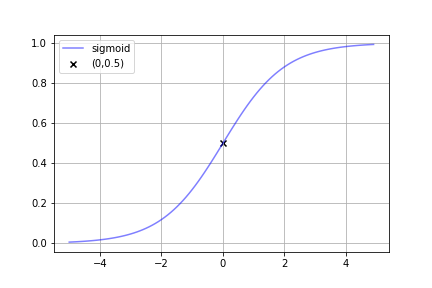
\includegraphics[scale=0.7]{sigmoid}
  \captionof{figure}{Graph of the sigmoid function}
  \label{fig:sigmoid}
\end{center}

\subsection{Hypothesis}

\noindent
The unvectorized form of the hypothesis for a given example $i$ is:

\begin{align*}
& h_{\theta}(x^{(i)}) = g \left( \sum_{j=0}^{n} \theta_j * x_j^{(i)}  \right) \in \left]0, 1\right[  \\
& \\
& where \; g \; is \; the \; sigmoid \; function.
\end{align*}

The hypothesis can be interpreted as the probability that a new observation belongs to the positive class i.e. that $y=1$ given the value of its features i.e. given $x$, parameterized by $\theta$. In other words:

\begin{equation}
h_{\theta}(x) = P\left(y=1|x;\theta \right)
\end{equation}

We then introduce the following decision rule:

\begin{equation}
y = 
\begin{cases}
1 & \text{if } h_{\theta}(x) \geq 0.5 \\
0 & \text{if } h_{\theta}(x) < 0.5
\end{cases}
\end{equation}

Finally, the vectorized form of the hypothesis can be written as follows:

\begin{align*}
& h_{\theta}(X) = g\left(X\theta\right) \in \left]0, 1\right[^{m} \\
& \text{where g is the sigmoid function applied element-wise}
\end{align*}

\subsection{Cost function}

Before introducing the cost function, let study two functions:

\begin{align*}
& v \; : \; x \in \left] 0, 1 \right[ \longrightarrow  -ln(x) \in \left[0, +\infty\right[ \\
& \\
& w \; : \; x \in \left] 0, 1 \right[ \longrightarrow  -ln(1-x) \in \left[0, +\infty\right[ \\
\end{align*}

Function $v$ has the following properties on the interval $\left] 0, 1 \right[$ :

\begin{itemize}
\item It is decreasing.
\item It converges to $+\infty$ in 0.
\item $v(1)=0$.
\end{itemize}

Function $w$ has the following properties on the interval $\left] 0, 1 \right[$ :

\begin{itemize}
\item It is increasing.
\item It converges to $+\infty$ in 1.
\item $w(0)=0$.
\end{itemize}

Here is the graph of $v$ and $w$ on the interval $\left] 0, 1 \right[$ :

\begin{center}
  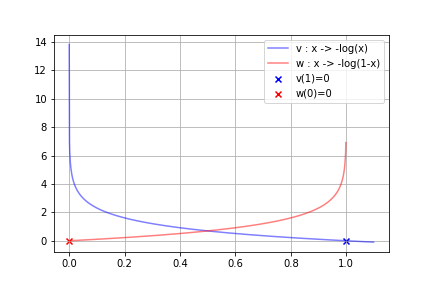
\includegraphics[scale=0.7]{vw}
  \captionof{figure}{Graph of $v$ and $w$}
  \label{fig:vw}
\end{center}

Now we introduce the following cost function:

\begin{align*}
& J(\theta) = \frac{1}{m} * \sum_{i=1}^{m} Cost\left(h_{\theta}\left(x^{(i)}\right), y^{(i)}\right) \in \mathbb{R} \\
& \text{where} \\
& Cost\left(h_{\theta}\left(x^{(i)}\right), y^{(i)}\right)  =
\begin{cases}
-ln\left(h_{\theta}\left(x^{(i)}\right)\right) & \text{ if } y^{(i)}=1 \\
-ln\left(1-h_{\theta}\left(x^{(i)}\right)\right) & \text{ if } y^{(i)}=0
\end{cases}
\end{align*}

Given that $y \in \{0, 1\}$, the cost function can be rewritten as:

\begin{equation}
J(\theta) = \frac{1}{m} * \sum_{i=1}^{m} \left[  \left(y^{(i)} * -ln\left(h_{\theta}\left(x^{(i)}\right)\right)\right) + \left( (1-y^{(i)}) * -ln\left(1-h_{\theta}\left(x^{(i)}\right)\right)  \right) \right] \in \mathbb{R}
\end{equation}

We can also write the vectorized form of the cost function as follows:

\begin{align*}
& J(\theta) = -\frac{1}{m} * \left[y^{\top} ln(h_{\theta}(X)) + (1-y)^{\top}ln(1-h_{\theta}(X)) \right] \in \mathbb{R} \\
& \\
& \text{where } ln \text{ is applied element-wise} 
\end{align*}

\subsection{Gradient descent}

The unvectorized form of the gradient of the cost function can be written as:

\begin{equation}
\frac{\partial J(\theta)}{\partial \theta_{k}} = \frac{1}{m} * \sum_{i=1}^{m} \left( \frac{1}{1+exp(-\sum_{j=0}^{n} x_{j}^{(i)}*\theta_{j})} - y^{(i)} \right) * x_{k}^{(i)} \in \mathbb{R}
\end{equation}

The vectorized form of the gradient of the cost function can be written as:

\begin{align*}
& \nabla J(\theta) = \frac{1}{m} * X^{\top}\left( h_{\theta}(X)-y \right) \in \mathbb{R}^{n+1} \\
& \\
& \text{where } h_{\theta}(X) \in \left]0, 1 \right[^{m} \\
\end{align*}

Denoting $\alpha$ the learning rate, a vectorized implementation of the gradient descent can thus be written as:

\begin{align*}
& \theta := \theta - \frac{\alpha}{m} *X^{\top}\left( h_{\theta}(X)-y \right) \in \mathbb{R}^{n+1} \\
& \\
& \text{where } h_{\theta}(X) = g(X\theta ) \in \left] 0, 1 \right[^{m} \\
& \\
& \text{and g is the sigmoid function applied element-wise}
\end{align*}

\subsection{Regularization}

The regularized cost function can be written as:

\begin{align*}
& J(\theta) = -\frac{1}{m} * \left[y^{\top} ln(h_{\theta}(X)) + (1-y)^{\top}ln(1-h_{\theta}(X)) \right] +\frac{\lambda}{2m}*\theta_{r}^{\top}\theta_{r}  \in \mathbb{R} \\
& \\
& \text{where } ln \text{ is applied element-wise} 
\end{align*}

The regularized gradient can be written as:

\begin{align*}
& {\left [ \widetilde{\nabla J(\theta)} \right]}_{1} = {\left [ \nabla J(\theta) \right]}_{1} \text{for } \partial \theta_{0} \text{ i.e. the first element of the regularized gradient} \\
& {\left [ \widetilde{\nabla J(\theta)} \right]}_{j} = {\left [ \nabla J(\theta) + \frac{\lambda}{m}*\theta \right]}_{j} \text{where } j \in \{2, 3, ..., n\}
\end{align*}

\section{Neural network classifier}
\subsection{Notations}

Let consider the following neural network:

\begin{center}
  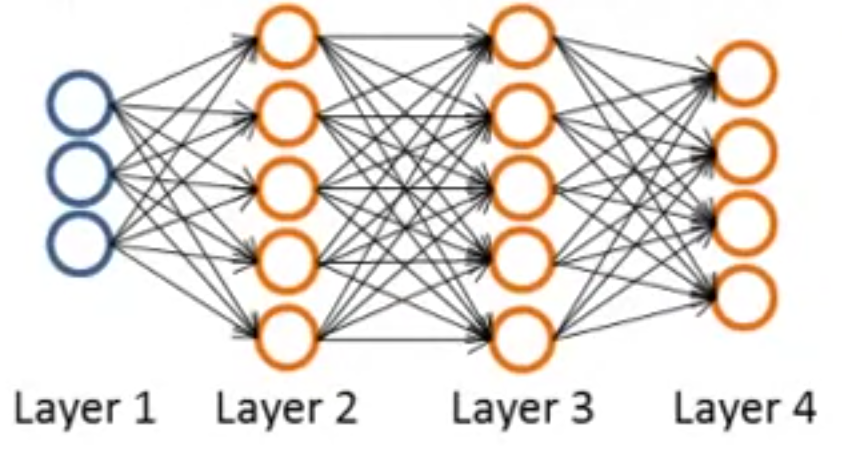
\includegraphics{neural}
  \captionof{figure}{Example of neural network}
  \label{fig:neural}
\end{center}

We assume that we face a multi-class classification where we want to predict whether an observation belongs to one of $K$ possible classes. We denote $L$ the total number of layers in the network. In the example, there are 4 layers. The first layer is called the input layer. The last layer is called the output layer. Intermediate layers are called hidden layers. Here, there are 2 hidden layers. We denote $s_{l}$ the number of units in layer $l$, not counting the bias unit. In the example, we thus have:

\begin{itemize}
\item $s_{1} = 3$ which is $n$, the number of input features.
\item $s_{2} = 5$.
\item $s_{3} = 5$.
\item $s_{4} = 4$ which is $K$, the number of classes.
\end{itemize}

We assume that a bias unit is added as an input to any layer.

We denote $m$ the total number of examples in our training set. We denote $x^{(i)} \in \mathbb{R}^{\left(s_{1} + 1 \right)}$ the vector of features of the $i-th$ example in the training set where $x_0^{(i)} = 1$. We denote $y^{(i)} \in \mathbb{R}^{K=s_{L}}$ the output vector of the $i-th$ example in the training set. If the $i-th$ example belongs to class $k$, then:

\begin{equation}
y^{(i)} = \begin{pmatrix} 0 \\ ... \\ 0 \\ 1 \\0 \\ ... \\ 0 \end{pmatrix} \text{where } {\left(y^{(i)} \right)}_{k, 1} = 1 \in \mathbb{R}^{K=s_{L}} 
\end{equation}

Note that the full output values can be stored in a matrix:

\begin{equation}
Y =  \begin{pmatrix} {y^{(1)}}^{\top} \\ ... \\ {y^{(m)}}^{\top} \end{pmatrix} \in \mathbb{R}^{m*K}
\end{equation}


Finally, we denote $\Theta^{(l)}$ the matrix of parameters required to go from layer $l$ to layer $(l+1)$. This matrix is in the space $\mathbb{R}^{s_{(l+1)} * \left((s_{l}) + 1\right)}$ since it maps vectors of dimension $((s_{l}) + 1)$ (do not forget the bias unit) into vectors of dimension $s_{(l+1)}$. Note that:

\begin{equation}
 \Theta^{(l)} =  \begin{pmatrix}  \text{Parameters associated to unit 1 of layer } (l+1) \\ ... \\ \text{Parameters associated to unit } s_{l+1} \text{of layer } (l+1) \end{pmatrix} \in \mathbb{R}^{s_{(l+1)} * \left((s_{l}) + 1\right)}
\end{equation}

In other words, ${\left(\Theta^{l}\right)}_{i, j}$ corresponds to the parameter associated to unit $j$ of the layer $l$, which is used to compute unit $i$ of the layer $(l+1)$. Note that in this example, there are 3 matrices of parameters to estimate : $\left(\Theta^{1}\right)$, $\left(\Theta^{2}\right)$ and $\left(\Theta^{3}\right)$. It implies $5*3 + 5*5 + 4*5 = 15 + 25 + 20 = 60$ parameters to estimate. In general, there are $(L-1)$ matrices of parameters to estimate. 

\subsection{Hypothesis}

The hypothesis can be written recursively as follows:

\begin{align*}
& X_1 = \text{the data matrix} \in \mathbb{R}^{m * (s_1+1)} \\
& \\
& X_{l+1} = 1_{m*1} \: \| \: g(X_{l}{\Theta^{(l)}}^{\top})  \in \mathbb{R}^{m * \left((s_{l+1})+1)\right)} \\
& \\
& h_{\Theta}(X_{1}) = g(X_{L-1}{\Theta^{(L-1)}}^{\top})  \in \mathbb{R}^{m * s_{L}} \\
& \\
& \text{where } \| \text{ means horizontal concatenation and } g \text{ is the sigmoid function applied element-wise}.
\end{align*}

Again, the hypothesis only gives the probability that an observation belongs to each class. As for the one vs. all multi-class classification problem, we then introduce the following decision rule to pick the most probable class given the input features:

\begin{equation}
\text{Class of } y = index_{of}\left( max_{row \: wise}(h_{\Theta}(X_{1})) \right) \in \mathbb{R}^{m}
\end{equation}

\subsection{Cost function}

Very similar to the cost function for the logistic regression, we just add a cost for the estimation of each output unit (now there are K of them). We also directly introduce the regularization term. Here is an unvectorized expression of the cost function:

\begin{equation}
\begin{split}
J(\Theta) = -\frac{1}{m} * \sum_{i=1}^{m} \sum_{k=1}^{K} y_{k}^{(i)} * ln({h_{\Theta}(X_{1})}_{i,k}) + (1-y_{k}^{(i)}) * ln(1-{h_{\Theta}(X_{1})}_{i,k}) \\
+ \frac{\lambda}{2m} * \sum_{l=1}^{L-1} \sum_{i=1}^{s_{(l+1)}} \sum_{j=2}^{(s_{l})+1} {\Theta^{(l)}_{i,j}}^{2}
\end{split}
\end{equation}

It can be vectorized as follows:

\begin{align*}
& J(\Theta) = -\frac{1}{m}  * \left[ \; Tr \left(ln(h_{\Theta}(X_{1}))Y^{\top}\right) + Tr\left(ln(1-h_{\Theta}(X_{1}))(1-Y)^{\top} \right) \; \right] \\
& + \frac{\lambda}{2m}*\sum_{l=1}^{L-1}Tr\left({\Theta_{r}^{(l)}}^{\top}\Theta_{r}^{(l)}\right) \\
& \text{where } \Theta_{r}^{(l)} = \Theta^{(l)} \text{ without the first column of }\theta_0s, \\
& \text{and }  h_{\Theta}(X_{1}) \in \mathbb{R}^{m*K} \text{ and } Y \in \mathbb{R}^{m*K}, \\
& \text{and } Tr(.) \text{ is the trace of a square matrix operator i.e. the sum of its diagonal}, \\
& \text{ln(.) is applied element-wise}. 
\end{align*}

\subsection{Backpropagation algorithm}

In order to minimize the cost function, we need to compute the partial derivatives of $J(\Theta)$ with respect to all the parameters i.e. with respect to each element of the $(L-1)$ matrices of parameters:

\begin{equation}
\frac{\partial J(\Theta)}{\partial \Theta_{i, j}^{(l)}} \text{ for } i, \: j, \: l
\end{equation}

To do so, we can use the backpropagation algorithm. This algorithm will yields the partial derivatives of $J(\Theta)$ with respect to each element of the matrices of parameters. 

\begin{itemize}
\item Step 1: Initialization. Set the matrices of parameters to random small values.
\item Step 2: Compute forward the activation of the units of each intermediate layer as well as the hypothesis i.e. the output units with matrices of zeroes.
\item Step 3: Compute the error of the last layer.
\item Step 4: Compute backward the errors of all previous layers until the first intermediate layer.
\item Step 5: Use the errors of each layer to compute the gradients of each matrix of parameters.
\end{itemize}


On the full sample, the errors can be computed as follows:

\begin{align*}
& \delta^{(L)} = A^{(L)} - Y^{(L)} \in \mathbb{R}^{m\times s_{L}} \\
& \delta^{(l)} =  \delta^{(l+1)} \Theta^{(l)} \: .* A^{(l)} .* (1-A^{(l)}) \in \mathbb{R}^{m\times (s_{l}+1)} \\
& \text{where } A^{(l)} = 1_{m*1} \: \| \: g(\Theta^{(l-1)}X_{l-1}^{\top}) 
\end{align*}

Finally, we can obtain the gradients as follows:

\begin{align*}
& \Delta^{(l)} = \frac{1}{m} * {\delta^{(l+1)}}^{\top}A^{(l)}  + \frac{\lambda}{m} * \Theta_{r}^{(l)} \\
& \text{where } \Theta_{r}^{(l)} = \begin{pmatrix} 0 \\ 0 \\ ... \\ 0 \end{pmatrix} \: \| \: \left[\Theta^{(l)}\right]_{col 2-end}
\end{align*}

Note that for $l=1$, we have $A^{1}=X$.

\section{Support Vector Machines}

\subsection{Hypothesis}

Support Vector Machines or SVM is another classifier.  The hypothesis is a discriminant function based on the value of the linear combination:

\begin{align*}
& h_{\theta}(x^{(i)}) = 
\begin{cases}
1 & \text{if } \theta^{\top}x^{(i)} >= 0 \\
0 & \text{otherwise} 
\end{cases}
& \\
& \text{where } x^{(i)} \in \mathbb{R}^{(n+1)} \text{ and } \theta \in \mathbb{R}^{(n+1)}
\end{align*}

\subsection{Cost function}

The cost function is inspired by the cost function of the logistic regression but is slightly different:

\begin{equation}
J(\theta) = C * \left[ \sum_{i=1}^{m} y^{(i)} * cost_1(\theta^{\top}x^{(i)}) + (1-y^{(i)})*cost_0(\theta^{\top}x^{(i)}) \right] + \frac{1}{2} \sum_{j=1}^{n} \theta_{j}^{2}
\end{equation}

Compared to the cost function of the logistic regression:

\begin{itemize}
\item We have dropped the $\frac{1}{m}$ factors
\item We have replaced the parameter $\lambda$ by a parameter $C = \frac{1}{\lambda}$. The bigger C, the more we want to fit exactly the data. The lower C, the more we want the parameters to be small.
\item The individual cost function assigning a cost to the prediction is the Hinge loss function.
\end{itemize}

It can be written in a vectorized form as follows:

\begin{align*}
& J(\theta) = C * \left[ (Y^{\top}cost_1(X\theta)) + ({(1-Y)}^{\top}cost_0(X\theta)) \right] + \frac{1}{2}*\theta_{r}^{\top}\theta_{r} \in \mathbb{R} \\
& \text{where } \theta_{r} \text{ is equal to } \theta \text{ without } \theta_0 \text{ thus } \in \mathbb{R}^{n} \\
& cost_0(.) \text{ and } cost_1(.) \text{are applied element-wise}.
\end{align*}

\subsection{Hinge loss functions}

For $y^{(i)}=1$, the hinge loss function is:

\begin{equation}
cost_1(z) = 
\begin{cases}
0 & \text{ if } z >= 1 \\
k(1-z) &  \text{ if } z<1
\end{cases}
\text{with k an arbitrary slope parameter } >0
\end{equation}

For $y^{(i)}=0$, the hinge loss function is:

\begin{equation}
cost_0(z) = 
\begin{cases}
0 & \text{ if } z < -1 \\
k(1+z) &  \text{ if } z>=-1
\end{cases}
\text{with k an arbitrary slope parameter } >0
\end{equation}

Here is a graph of $cost_0$ and $cost_1$ on $[-2,2]$ with $k=2$:

\begin{center}
  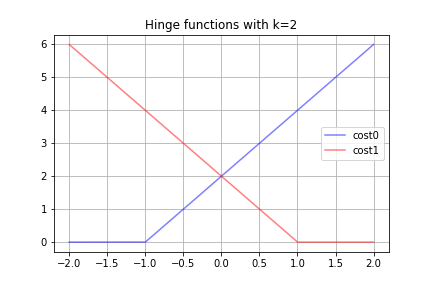
\includegraphics[scale=0.7]{hinge}
  \captionof{figure}{Graph of $cost_0$ and $cost_1$ with $k=2$}
  \label{fig:hinge}
\end{center}


\subsection{Large margin intuition}
 
When ...


\end{document}